\documentclass[12pt,final,oneside]{fithesis}
\usepackage[slovak,english]{babel}
\usepackage[T1]{fontenc}
\usepackage{makeidx}
\usepackage{graphicx}
\usepackage{lmodern}
\usepackage{url}
\usepackage{caption}
\usepackage{listings}
\usepackage{color}
\usepackage{xcolor}
\usepackage[pdftex,bookmarks=true]{hyperref}
\usepackage{paralist}
\usepackage{textcomp}
\usepackage{enumitem}
\usepackage[absolute]{textpos}

\clubpenalty=300
\widowpenalty=300

\hyphenation{da-ta-base hy-po-nym me-ro-nym me-ta-da-ta HTMLCleaner}

% syntax highlighting

\newcommand{\bb}[1]{\textbf{#1}}
\newcommand{\code}[1]{\emph{#1}}
\newcommand{\n}{\lstinline|\n|}

\definecolor{javared}{rgb}{0.6,0,0} % for strings
\definecolor{javagreen}{rgb}{0.25,0.5,0.35} % comments
\definecolor{javapurple}{rgb}{0.5,0,0.35} % keywords
\definecolor{javadocblue}{rgb}{0.25,0.35,0.75} % javadoc
\definecolor{bashnormal}{rgb}{0.0,0.0,0.0} % bash

\lstdefinestyle{command} {
	language=bash,
	basicstyle=\ttfamily\small,
	keywordstyle=\color{bashnormal}\bfseries,
	stringstyle=\color{javared},
	commentstyle=\color{javagreen},
	numbers=none,
	numberstyle=\tiny\color{black},
	stepnumber=1,
	numbersep=5pt,
	tabsize=2,
	showspaces=false,
	showstringspaces=false,
	breaklines=true,
	captionpos=b
}

\lstset{style=command}

\lstdefinestyle{text} {
	language=bash,
	basicstyle=\ttfamily\small,
	keywordstyle=\color{bashnormal}\bfseries,
	stringstyle=\color{javared},
	commentstyle=\color{javagreen},
	numbers=none,
	numberstyle=\tiny\color{black},
	stepnumber=1,
	numbersep=5pt,
	tabsize=2,
	showspaces=false,
	showstringspaces=false,
	breaklines=true,
	captionpos=b
}

\lstset{style=text}

\lstset{
	language=XML,
	basicstyle=\ttfamily\small,
	keywordstyle=\color{blue},
	stringstyle=\color{black},
	commentstyle=\color{javagreen},
	morecomment=[s][\color{javadocblue}]{<!--}{-->},
	morekeywords={project},
	identifierstyle=\color{black},
	numbers=left,
	numberstyle=\tiny\color{black},
	stepnumber=1,
	numbersep=5pt,
	tabsize=2,
	showspaces=false,
	showstringspaces=false,
	breaklines=true,
	captionpos=b
}

\lstset{
	language=Java,
	basicstyle=\ttfamily\small,
	keywordstyle=\color{javapurple}\bfseries,
	stringstyle=\color{javared},
	commentstyle=\color{javagreen},
	morecomment=[s][\color{javadocblue}]{/**}{*/},
	numbers=left,
	numberstyle=\tiny\color{black},
	stepnumber=1,
	numbersep=5pt,
	tabsize=2,
	showspaces=false,
	showstringspaces=false
	breaklines=true
	captionpos=b
}

\makeindex

\thesistitle{Arquillian testing platform support for Android web and native applications}
\thesissubtitle{Diploma thesis}
\thesisstudent{\foreignlanguage{slovak}{Bc. \v{S}tefan Miklo\v{s}ovi\v{c}}}
\thesiswoman{false}
\thesisfaculty{fi}
\thesisyear{spring 2013}
\thesisadvisor{RNDr. Adam Rambousek}
\thesislang{en}

\begin{document}

\FrontMatter
\ThesisTitlePage

\newpage
\thispagestyle{empty}
\begin{textblock*}{\paperwidth}(0mm,0mm)
   \noindent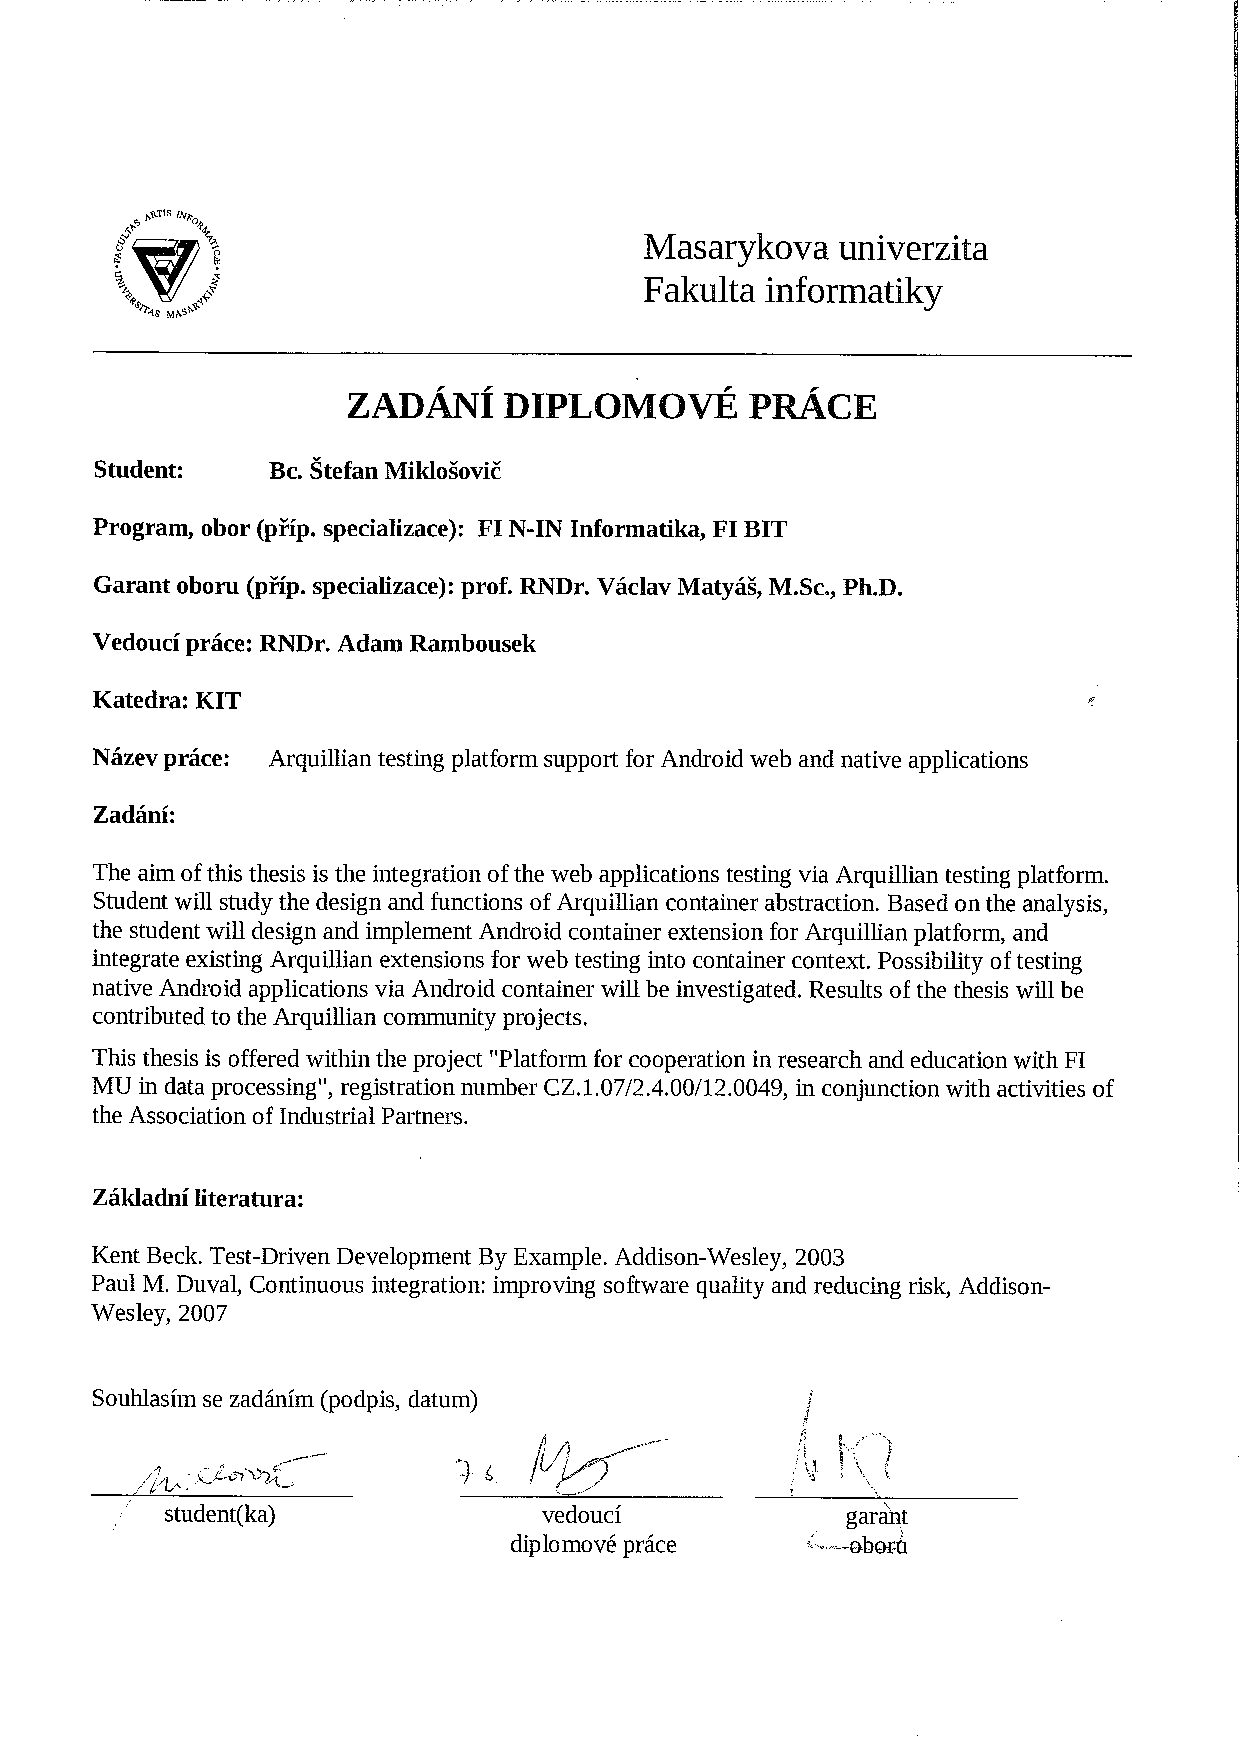
\includegraphics[width=\paperwidth,height=\paperheight]{resources/zadanie.pdf}
\end{textblock*}
\mbox{}\newpage

\begin{ThesisDeclaration}
\DeclarationText
\AdvisorName
\end{ThesisDeclaration}

\begin{ThesisThanks}
I would like to thank Karel Piwko, my leader in Red Hat Inc., for his valuable advices and insights during writing this thesis which helped me to understand the internal working of Arquillian framework a lot better. My thanks are going to Aslak Knutsen from Red Hat Inc. for the similar reasons.
\end{ThesisThanks}

\begin{ThesisAbstract}
The aim of this thesis is to design and implement an Arquillian container for Android devices, which is used during functional tests of web applications running at enterprise application servers. Investigation of functional testing of native Android applications via implemented Arquillian Android container is presented.

This thesis is offered within the project ''Platform for cooperation in research and education with FI
MU in data processing'', registration number CZ.1.07/2.4.00/12.0049, in conjunction with activities of
the Association of Industrial Partners.
\end{ThesisAbstract}

\begin{ThesisKeyWords}
Arquillian, container, Android, ShrinkWrap, testing, functional, integration, extension, JBoss, enterprise, Drone, JavaEE, Maven, JUnit
\end{ThesisKeyWords}

\clearpage
\thispagestyle{plain}
\par\vspace*{.35\textheight}{\textit{Identical units tested under identical conditions will not be identical on the final test after being buried under other components and wiring.} {\par}\hfill{Murphy's law}}

\MainMatter
\tableofcontents

\chapter{Introduction}
The result of one's activity in the manner of a tool or an application, which is to be used by him or by others, in order to be helpful and to fulfill the specified aim and before its introduction to production, has to be tested.

In context of the Murphy's law at the beginning of this thesis, we could ironically say that it holds in software engineering very strongly. Software engineering and development of software as such strives for quality in sense of absence of bugs and smooth integration into existing solutions or functionality of the product.

Quality engineering and testing methodologies in Java enterprise environment have been the subject of very vivid discussions. Couple of techniques as unit testing by testing frameworks as JUnit, TestNG and others have emerged and whole concept of programming like test driven development or eXtreme Programming have been propagating widely. 

Besides the unit testing as the very basic principle of testing, integration and functional testing is as important as the former one. In the zoo of frameworks and plethora of tools for Java EE platform, it is important to be sure not only components of the software solution work as expected but also their interconnection, communication and integration with enterprise application containers and other enterprise layers is functioning as well.

While trying to doing so, we realize very early that it is not easy task and in lot of cases not even possible. The reason why is that we are are trying to bring the whole runtime into our tests so we are orchestrating all layers trying to fake the target environment in which our product will be running. The mocking and faking of all complex enterprise services as dependency injection, messaging or database performance and simulating system errors and communication between multiple entities in our software solution is heroic work and it is not possible to simulate exactly the same scenario multiple times and repeatedly.

This thesis aims to improve functional and integration testing of web and native Android applications on JBoss platform cooperating with Android platform. The crucial role in the functional and integration testing plays Arquillian testing platform.

Arquillian testing platform provides a way by which we can get rid of aforementioned impossibilities of testing cases. The core principle which stands behind Arquillian is the philosophy of bringing tests into target runtime and not otherwise - the typical way of dealing with tests so far. The imple switching of point of view makes whole enterprise testing in Java EE revolutionary. 

It is important to realize the essential component without which testing by Arquillian would be meaningless - application container or application server. The application container is a place where, roughly speaking, application is deployed and made accessible for clients. Arquillian is container agnostic, which means it does not matter against what target environment the application is tested.

Arquillian is not only a tool for rigid testing of enterprise services and technologies but it also provides a way how to do testing by automating a web browser in case we are trying to test functionality of some web application. There are already solutions how to automate web browser such as via Selenium (and its successor named WebDriver)- the pioneer of automated testing frameworks. JBoss community developed a tool which is based on Selenium of name Arquillian Graphene. Arquillian Graphene is designed as set of extensions for Selenium WebDriver.

The functional testing by automating web browsers has its counterparts in Android platform, to name a few, Solo, Robotium or Selendroid. This thesis tries to focus on integrating these kind of tools into Arquillian environment. We try to make functional testing of Android applications as similar to web testing via Selenium as possible so we can gain from advantages of Arquillian in this direction too. 

\chapter{On software development processes}

In this chapter, we are discussing two most widely-known approaches to the development of the software - serial (or sequential) development model and iterative development model. Both models will be described and their pro et contra will be discussed. We will discuss both models in sense of their attitude to testing process or methodology too.

	\section{Serial development process}
	
Serial development model is the traditional software development process. This process is commonly used in the most software projects. The main description of the process is that it is divided into set of activities. When one set of activities is finished, the other one starts. When all sets of activities are done, the whole development process is considered to be about its end. The development model of such pattern is also called waterfall process since there is no easy way how to go back in the development and return to some previous stage. There is basically no way how to switch to the older stage or at least it is used to be challenging and more resource, time and finance demanding.

The process has typically five phases as it is shown in the next figure. To name them, they are called: requirement analysis, design, implementation, testing, installation and maintenance.\\

\begin{figure}
	\centering
	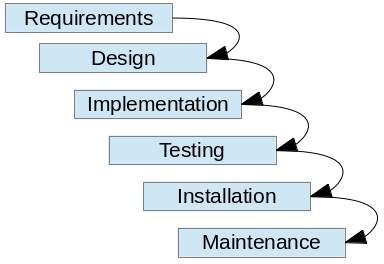
\includegraphics[width=70mm]{img/waterfall.png}
	\caption{Waterfall development process}
	\label{fig:waterfall_process}
\end{figure}

\begin{itemize}
	\item[\textbf{Requirements analysis:}] This step is the most important phase of the waterfall model. In this phase, all customer requirements are gathered, involving clear definition of the customer goals and expectations. Requirements analysis is also the place where the understanding of the customer's context and constrains are specified. To obtain all these information, the customer is involved into this phase very early and actively since he represents the only source of information which developers have the access to. The outcomes of the analysis are persisted to so called software requirement specification (SRS) of the application. The SRS is describing the behavior of the system entirely and in the great depth and detail. The SRS in used in the next phases frequently.
	\item[\textbf{Design:}] After SRS is available, software architects and designers are about to start the designing of the overall look of the software solution. The design phase involves defining the hardware and software architecture, specifying performance and security parameters, designing data storage containers and constraints, choosing appropriate IDE and programming languages and indicating strategies to deal with issues such as exception handling, resource management and interface connectivity. The output of this stage is called SDD - software design description.
	\item[\textbf{Implementation:}] After the final product is fully designed and all requirements of the customer were incorporated, the implementation of the product takes its place. The input to the implementation phase is the SDD of the system from the design phase. The implementation phase is the logical continuation of the design phase where the product is built.
	\item[\textbf{Testing:}] Testing phase, which follows the implementation phase, verifies that the application or the software solution is meeting requirements put on the product in the first phase and additionally that the application is free of bugs. The test cases are written in order to evaluate the implementation. There are various categories of testing - unit testing, system testing or acceptance testing and last but not least functional and integration testing. If some errors, bug or malfunction are observed, it is up to the development team to refactor the code, incorporate changes and do tests once again until the product is valid and ready to be installed.
	\item[\textbf{Installation:}] Installation phase actually delivers the developed and tested product to the customer. It can be installed by customer itself, by development team or by other third party.
	\item[\textbf{Maintenance:}] Waterfall model is finished by maintenance phase which follows installation phase at the client side. There is not any functionality added. This phase is used to tweak the product in a such way that its performance is improved and attributes of the product are modified to better reflect clients execution environment which are hard to estimate in advance.
\end{itemize}

To sum up the sequential (serial) development model, the main idea behind this kind of models is to design and project every single aspect of the final product in very deep details. Only after very careful specification of what is going to be done, further steps are taken, ignoring the client or customer from the development process, when all possible information are extracted. The reason of doing so is to reduce wasted time by avoiding the need to go back and to make corrections which are used to be costly.

The main disadvantage of this approach is that the never-go-back mentality of the serial process makes it very hard to maintain and build adaptable and modifiable code in the future. The sequential model tries to avoid changes while the product is being developed.

On the other hand, these types of development processes are suitable for projects where it is known keeping the room for changes in the future is not necessary or not required. In addition, having a precise idea of what application will consist of and what requirements are put on it can uncover notable flaws that might occur in later stages.

	\section{Iterative development process}

Iterative development processes can be viewed as direct opposite of sequential ones. Functionality is added by iterations, from very basic to more advanced, from simpler to more complex. In this section, we will discuss two approaches which are very popular among iterative development processes. Tests coders are preparing while they are developing the application is the activity which is in these days not considered to be only the side effect and the evil which has to be eventually done, but it is a way and strategy how to develop as such. This approach to the developing is called test driven development (TDD). Test driven development plays very nicely with another popular term which symbolizes whole principle of coding - eXtreme Programming (XP).

	\subsection{Test driven development}
	
Test driven development is a way of programming when we are writing your tests firstly and before any single line of code of the target application is written. The first step is to add quickly a test which has to fail upon first run. Only when a test is written, we write the application code and run that test against what is coded so far to get rid of failing test and have the test which passes. If we run the code and that code is still failing, we have to return back to coding, repair the code and run test once again. Only when tests are passing, we can write other tests which test different functionality and do the same process again.

The process just described is called TFD (test-first development). Test driven development is understood as a TFD with refactoring. This approach to programming process is completely different from what majority of programmers are used to. The traditional view is to code some subset of the functionality and then to write tests to see if it fails or passes and react accordingly. The importance of getting tests written in advance is in the way how we think about the design of the application. We are trying to make our design the best possible in advance thinking about how some particular design is going to be helpful for us. TDD calls for the opposite way. We are focusing on new functions so every other added functionality constantly improves our design and just fits our needs.

\newpage
There are two levels of TDD:

\begin{itemize}
	\item{\textbf{Acceptance TDD (ATDD):}} With this approach, we are writing single acceptance test and just enough production code to satisfy that test. The goal of ATDD is to specify detailed, executable requirements for our solution on a just in time (JIT) basis. ATDD is also called Behavior Driven Development (BDD).
	\item{\textbf{Developer TDD:}} With developer TDD we write a single developer test, sometimes inaccurately referred to as a unit test, and then just enough production code to fulfill that test. The goal of developer TDD is to specify a detailed, executable design for our solution on a JIT basis.  Developer TDD is often simply called TDD.
\end{itemize}

The result of programming TDD way can be summarized in these points:

\begin{itemize}
	\item{Our development environment must provide rapid response to small changes.}
	\item{Unit tests has to run fast (they have short setups, run times, and break downs).}
	\item{Unit tests run in isolation, we should be able to reorder them so no test is dependent on the other.}
	\item{Tests are using real data and are executed in simulated production environment.}
\end{itemize}	

	\subsection{Extreme Programming}
	
Extreme programming is one of the several popular agile processes. The extreme programming style of the software development is hard to describe in its entirety but in order to complete the image of how the programming can be and is done these days, we have to evaluate it.

What is one doing if he develops in the extreme way? To describe his attitude superficially, the first of all, so-called extreme developer starts to code as soon as possible and does not think about the overall design of the application in advance. At the first look, this basic strategy can appear to be dangerous, chaotic or even wrong at all from the academic point of view where sequential development strategies or waterfall-like strategies are used rather often, but this approach has some undeniable advantages and desirable consequences which are highly valuable and will be discussed.

When a developer team starts to work on some project, the very typi\-cal beginning is to plan everything into details and the significant amount of time is spent with the customer describing and specifying what output he wants to eventually see. The big problem of this app\-roach is the uncertainty of the output. With the best intentions to catch user's needs and requirements, nobody is able to be completely precise about how the final product will look like. It is not the fault of the development team, meaning its disability to understand what the customer wants. Typically, a customer or a consumer of an application even does not know what should be done. A customer is used to have only vague idea what kind of problem the application should solve and he is willing to change the goal, design and requirements as the application is evolving.

For these reasons, the typical scenario mentioned in the sequential models, which is to consult everything in advance, is flawed and not sufficient. It is often the case that after a customer declares what he wants and the consulting is done, the second time we face the customer is upon final delivery of the product. In the extreme programming paradigm, a customer is the essential part of the developing process and he is participating all the time application is under construction. Of course, one has to design and plan at least something, there has to be clear borders e.g. the problem domain the application will be dealing with, but every further details of how it should be done later are almost meaningless.

The extreme way of programming is also about doing plans but the strongest attitude can be sum up with the slogan "Do the Simplest Thing that Could Possibly Work" and the abbreviation \textit{YAGNI} which stands for "You Are not Going to Need It".

While the meaning of the first phrase is clear, the mentioned abbreviation has to be clarified. When we are developing the application, we are very often ending up with the design which is over-engineered. After completion of some problem, we have coded infrastructure for solving problems which do not even exist yet and we provided functionality which is not necessary. We likely think that by coding a lot in advance, we will be free from implementing it once there will be the need to do so. We are keeping doors widely open to hook and modify almost everything or at least with the smallest pain. But the question is - what if that situation never happen? By implementing the functionality we do not need, we will face two very probable outcomes. The~first is the need of taking care of the unused code and pulling it all the way with us while we develop which adds additional complexity to the existing code and by this way it becomes more error prone. The second is the fact that our imagination of what user wants is completely out of range so we are wasting the time.

The key concepts of the extreme programming can be summed up in the following points:
\begin{itemize}
	\item make frequent and small releases
	\item a project is divided into iterations
	\item no functionality is added early
	\item refactor whenever and wherever possible
	\item code the unit test first
	\item integrate often
	\item all code must have unit tests
	\item when a bug is found, tests are created
\end{itemize}   

Extreme programming suffers from some drawbacks too. Extreme programming is more code-centered then design-centered so it is more suitable for smaller projects or in projects which do not span over more development teams. Using extreme programming in such scenario would be more counterproductive than useful. Since extreme programming lacks design documentation in great detail because it varies constantly, we are short of reuse opportunities. Extreme programming does not maintain quality plan. Having of such plan reduces time reserved for testing. Extreme programming spends huge amount of time on testing process. 

In spite of mentioned drawbacks, extreme programming can be successful because it focuses on the customer's satisfaction in every moment. We could be aware that some feature will be needed in the future but we are not going to implement it right now even it is very easy to introduce and implement - it is not necessary at the present moment. When the time comes, the code can be refactored and missing functions added and it does not matter if we are in the late period of the life cycle of the product or not. The architecture and design of the project or its part is kept as simple as possible so further modifications and additions can be done over the skeletal design - enabling continuous refactoring.

	\section{Necessity of continuous integration}
	
Both models of software developing we discussed earlier - sequential development process which is the representative of the waterfall model and iterative development models as TDD and XP - have to integrate the functionality and code into the already existing code base.

While in the sequential development process the integration phase is standalone, long term and time consuming event, it is often only the bad practice and habit why it is so. The key to the successful and painless development scenario is to integrate part by part, code by code and day by day as iterative approach suggests. This approach is rarely taken in the case of sequential development. On the other hand, TDD and XP approach is very suitable for so called continuous integration. We will describe what continuous integration (CI) is and how can be helpful in both development models mentioned in the previous sections.

We can explain continuous integration process on the example in context of XP as well as waterfall on the next figure:

\begin{figure}
	\centering
	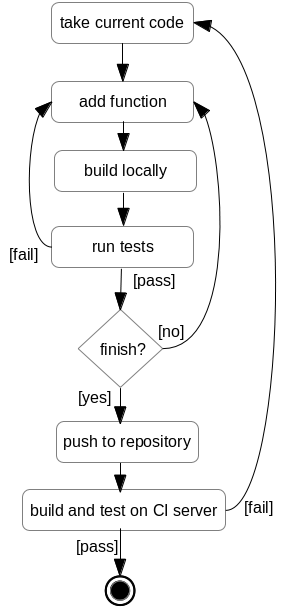
\includegraphics[width=70mm]{img/ci.png}
	\caption{Continuous integration}
	\label{fig:ci_process}
\end{figure}

\newpage

The very first goal in order to do CI is to have a central place where the all source code and resources necessary to build and run the project are stored. It is important to realize that a source code repository should contain everything needed in order to build the project successfully - not only source code itself but whole tools, scripts and resources. In the ideal state, we should check out the code from the repository on the clean (developer) machine and run tests, build application and run it from scratch. The most popular distributed source code repository nowadays is Git\footnote{http://git-scm.com/}, so the reader can bear in mind this kind of repository while reading further.

When a developer clones a repository or when he updates his local repository to the newest commit to synchronize his local repository with the main repository, he starts to add a functionality into the code. It does not matter what kind of functionality or change it really is, but let's say, for the sake of the argument, he is trying to add some business functionality or fulfill some user's story card.

While doing so, he writes tests, as the TDD approach is advising, builds the project locally, ensures himself that tests which verify new functionality are failing and starts to implement what is necessary.

He builds the whole project or module of the application as he develops, checking his progress. He repeats this process while tests are failing. When they stop to do so, it is the sign that the functionality is implemented and he can commit and push to the remote repository where everybody checks the source code from.

By committing to the remote repository, his work is done only partially. It is so because there is a continuous integration server which fetches the whole repository, builds the project and runs all tests again.

The necessity of continuous integration server is determined by distributed nature of the source code repository. More then one developer can check the source code so more then one developer can work on the project simultaneously which means that after both developers commit their work, after resolving possible clashes which originate from the work of both of them, we have to build and test once again since there can be still a possibility that some artifacts or resources are not pushed to the repository so build which is run externally from development machine can fail.

Activities related to the continuous integration can be handled automatically or manually. Automatic builds can be executed on some preferred interval or when changes in the main repository are detected.

After getting the initial image of the CI, when one wants to use CI, he needs to build and maintain an infrastructure which: \textbf{ref na fowllera}

\begin{itemize}
	\item{contains a single source repository}
	\item{automates builds}
	\item{makes builds self-testing}
	\item{builds the newest code on the integration machine}
	\item{keeps builds fast}
	\item{tests in production environment}
\end{itemize}

As mentioned earlier, source code can be tracked in Git but other source code repositories can be used as SVN\footnote{http://subversion.apache.org/} or Mercurial\footnote{http://mercurial.selenic.com/}.

It is clear that the main stress will be put on the fact that the builds and tests have to be done fast because they are done frequently. If our builds or functional and integration tests took tens of minutes or hours, it would be useless to use the TDD and XP in the Java EE environment. Tests are driving the development. Testing \emph{is} development. We are doing incremental changes, we are adding functionality frequently and piece by piece and we also integrate on-the-fly so we know better every moment how is our project doing which is only hardly doable in the sequential development model when the integration exhibits at the end of the implementation when the refactoring of the code is very hard. Continuous integration process encourages to do smaller steps and to check how successful we are, keeping the overview of the project up to date.

We are also trying to run all tests in the target environment so we need take our tests to the runtime and not otherwise as it was discussed in the previous sections.

\chapter{Testing in Java EE environment}

In the last chapter, we described development processes of various qualities and we made stress on the importance of XP and TDD. The next chapter will discuss existing tools and techniques which are used in connection with testing process described earlier. We are dividing these tools which will help us to describe the context of Arquillian testing into three categories. These tools and software compilations are helpful for ongoing explanation of Arquillian testing platform and the reader will be prepared to understand the whole model of Arquillian testing, in connection with XP, TDD and CI, much better and smoother.

	\section{Tools used in JavaEE environment}
	
		\subsection{Maven}

Maven is so-called build automation tool. Maven is written in Java programming language and it is massively used in Java ecosystem. The main purpose of Maven is to describe the software project - its build, its development, testing and release life cycle and other projects on which our project is dependent with version management in mind.

By default, for every Maven-based project, the structure of directories is the same for all of them. 
In source-related directories, Java packages are saved. The default directory layout for a project is as follows:

\lstinputlisting[style=text,caption=A Maven project directory layout]{src/maven_layout.txt}

A typical Maven build life cycle consists of sequence of phases - \texttt{prepare-resources},\texttt{compile},\texttt{package},\texttt{install}. There are always \texttt{pre} and \texttt{post} phases which can be used to register \texttt{goals} which must run prior or after a particular phase.

Maven has following three predefined life cycles - \texttt{clean}, \texttt{default} and \texttt{site}. The \texttt{clean} life cycle cleans a project, the \texttt{default} life cycle builds a project and the \texttt{site} life cycle builds complete web site representation of a project into \texttt{target} directory, for example it generates Java documentation (javadocs).

A \texttt{goal} represents a specific load of work a plugin has to execute and doing so contributes to the building and managing of a project. The order of goals is defined by default settings which could be overridden~- we can easily define our own actions which are executed upon the build of the project. The order of execution depends on the order we specify phases and goals on the command line.

Maven is mostly ridden by command line command \texttt{mvn} after which phases and goals follow. Phases and 
goals can be chained. A goal of some plugin can be executed as:

\lstinputlisting[style=command]{src/maven_execution.sh}

For example, when we want to clean the project (to delete the build) we have to trigger \texttt{clean} phase. By default, the \texttt{clean} phase deletes \texttt{target} directory. If we want to build sources and make a \texttt{jar} package, we need to invoke \texttt{package} phase. Since goals can be chained, we execute:

\lstinputlisting[style=command]{src/maven_clean_package.sh}

When specifying \texttt{package} phase, all goals and phases which proceed this phase are executed as well. For example, \texttt{test} phase is executed after \texttt{compile} phase but before \texttt{package} phase, so we are sure tests are executed and software does what it is supposed to do before packaging is carried out.

The second very important role of Maven is to track \textit{dependencies}. Dependencies are stored in \textit{repositories}. By default, dependencies are downloaded from main Maven repository\footnote{http://search.maven.org/}. After downloading dependencies we need to satisfy our project with, they are stored in a cache repository at a development computer so that way there is no need to download them over and over again. A dependency is an \textit{artifact} which has exact and unique \textit{Maven coordinates} over all dependencies. Every artifact has coordinates of the form:
\begin{center}
	\begin{minipage}{.7\textwidth}
		\lstinputlisting[style=command]{src/dependency_coordinates}
	\end{minipage}
\end{center}
Every artifact belongs to some \textit{group}. This fact is reflected via \texttt{groupId} element. An artifact can have different \textit{versions}. We can not import two same dependencies each having different version. \texttt{packaging} element specifies how project is packaged. The most common values are \texttt{jar} or \texttt{pom}.

All project definition is stored in file called \texttt{pom.xml} which is the shortcut for \textit{project object management}. Maven finds \texttt{pom.xml} automatically when it is invoked in the same directory as \texttt{pom.xml} is saved. The very basic \texttt{pom.xml} file for the illustration purposes to reflect previously written is following:

\lstinputlisting[language=XML,label=pop-pipe,caption=A simple pom.xml file]{src/pom_example.xml}

A dependency can have a parent, in that case, project's \texttt{pom.xml} it is not a \textit{top-level} \texttt{pom.xml}. A parent normally serves as an aggregator of different dependencies which are logically grouped but each artifact has its own responsibility and specific meaning in a project. After parent definition, coordinates of an artifact follows and finally we see this artifact depends on \texttt{junit} artifact of particular version and \texttt{scope}. When \texttt{scope} is not defined, it means that dependency is on class path during compilation time. When \texttt{scope} is set to \texttt{test}, it means this dependency will be on class path only during testing phase of the project - when we execute Maven as \texttt{mvn test}.

In Maven universe, besides ordinary POM files, there are also so-called \textit{BOM} files. BOM stands for \textit{bill of materials}. It is a POM file where only dependencies are specified so we can easily include BOM dependency into \texttt{pom.xml} and all dependencies which are specified in BOM will be imported to \texttt{pom.xml} as well. We can gather well known group of dependencies and import only one dependency which covers them all in order to provide more brevity and management convenience.

Maven is very helpful tool which simplifies project management in Java EE environment enormously. Dependency tracking and artifact retrieving hide complexity of a project. The managing of a project life cycle would be very time demanding and daunting task since we would have to specify everything manually. 

	\subsection{ShrinkWrap}

ShrinWrap is very simple but powerful tool. ShrinkWrap is Java library which provides a mechanism for constructing archives as \texttt{jar}, \texttt{war} or \texttt{ear} programmatically and very easily. This is possible because of fluent API on which ShrinkWrap relies heavily and it is de facto the only way how to use the library. ShrinkWrap is standalone library and it does not depend on any additional artifacts. It needs just JRE5+ runtime.

The main reason for using ShrinkWrap is the easiness of creating custom archives. An archive file is built in a memory and written to any target location via so called \texttt{exporter} afterwards. Resources which are added to final archive are located on class path.

ShrinkWrap is very sought-after tool since we can exactly specify, class by class and resource by resource, how the deployment to application server will look like and drive very subtle class path isolation which is not so obvious every time. When we are creating an archive, it is common that resources and classes which are not needed are bundled into final package as well. This fact can negatively influence functionality and run time of a deployed package e.g. by not finding desired resources or because of some clash. While testing the software, we need to isolate test cases and find the smallest common denominator which satisfies all dependencies and we need to get rid of unused resources. This approach also encourages TDD and unit testing - we are only testing classes we are interested in and we are not taking any garbage  with us which could influence the results of the test unpredictably. The example of constructing \texttt{jar} file programatically via ShrinkWrap fluent API is following: 

\lstinputlisting[language=Java,label=pop-pipe,caption=ShrinkWrap fluent API]{src/shrinkwrap_archive.java}

The newly created \texttt{jar} file is stored in a generic \texttt{Archive} at line 5. The entry point for dealing with the library is \texttt{ShrinkWrap} class. We specify we want to create \texttt{JavaArchive}. This class has to extend generic \texttt{Archive} class (line 3). After these information, we are simply adding classes, packages or resources as manifest files into the archive, which will be persisted in \texttt{test.jar}.

Creating deployable archives with ShrinkWrap is very convenient way how to precisely specify and construct an archive which just meets our needs. We are able to put everything we want into the archive under the construction so we can bundle there our own resources at will as well as we can isolate or delete any resources and classes we want in order to strip an archive to bare deployable minimum.

		\subsection{Jenkins}

Jenkins in a continuous integration (CI) tool written in Java language. Jenkins is an open source project. The purpose of Jenkins is to provide continuous integration services for development of software. In its core, it is server-based system running in some kind of servlet container as Apache Tomcat\footnote{http://tomcat.apache.org/}.

Testing machines we are testing software under development at are called \textit{slave nodes}. A slave has various parameters such as amount of memory available, kind and version of operating system, system architecture, installed versions of Java Virtual Machines and so on. We can then register various integration servers at will and we can specify on which slave nodes we want to test our software according to their capabilities and our requirements. More often we do not specify directly which slave node we want to use. We only tag slave nodes by its capabilities and specify a query via which appropriate nodes are selected automatically.

Tests can be run at more then one slave node since we may want to know if our software is capable of running under various circumstances, e.g. if it works without issues on multiple configurations so we mimic heterogeneous target environment.

After the filtering on which node tests are going to be executed, the actual source code of our interest has to be checked out (or cloned) from central source code repository as Git\footnote{http://git-scm.com/}.

The building of tests can be triggered by various means, it can be triggered periodically on some predetermined frequency (e.g. every two hours) or it can be triggered automatically by every commit we push into source code repository. Jenkins uses concept of \textit{downstream} and \textit{upstream} builds so tests or builds of downstream project is triggered when all upstream projects are built and tested without issues. Local copy of source code is cloned at slave node and Jenkins executes tests and reports results back to Jenkins master server.

Jenkins plays significant role in Java EE environment and is very widely known to Java-oriented community. Jenkins performs very well in connection with Maven-based projects and it can test and build virtually any Java project. There is the effort to make various bindings to support .Net\footnote{http://www.microsoft.com/net} or Scala\footnote{http://www.scala-lang.org/} projects with various success.

Continuous integration system as Jenkins offers the very first prerequisite for successful and painless iterative development as described earlier and reduces uneasiness of integration testing significantly.

		\subsection{JUnit}
		
After having an arbitrary Java project based on Maven and setting up infrastructure for continuous integration testing via Jenkins, where source code is cloned or checked out from distributed source code repository, we need to perform testing itself. The most popular testing tool for Java is JUnit. JUnit is an instance of the xUnit architecture for unit testing frameworks.\footnote{http://junit.org/}.

JUnit tests, as the name of the framework suggests, are meant to be unit tests. As previously stated, in TDD model, which is often used in XP, unit tests are written before the code itself is created so only when tests are passed, code is considered to be finished. The very central point of the unit testing is to show that each part of the program behaves correctly. Only after that, these parts are integrated together.

JUnit is added to Maven-based project as a dependency. All tests reside by default in \texttt{src/test/java} and resources needed for tests under run, if any, are located in \texttt{src/test/resources}. From Maven point of view, tests are executed by \texttt{mvn test} command.

The example of simple JUnit test is following. Its core features and life cycle of the test class will be discussed further.

\newpage

\lstinputlisting[language=Java,label=pop-pipe,caption=Example of JUnit test]{src/ExampleTestCase.java}

A unit test is distinguished by JUnit when a test class is annotated with \texttt{@RunWith} annotation. Argument of \texttt{@RunWith} annotation is so-called \textit{test runner}. Test runner specifies how exactly test class, in our example \texttt{ExampleTestCase}, is treated. \texttt{JUnit4}\footnote{in org.junit.runners package} is the default runner for JUnit. It extends \texttt{BlockJUnit4ClassRunner} in the same package. Every runner has to extend this base runner. Custom JUnit runners are changing the default behavior of the test execution.

Every test case consists of particular test methods recognized by being annotated with \texttt{@Test}. All tests have to be \texttt{public void} methods without any arguments. The \texttt{@Test} annotation can have the argument \texttt{expected} which tells that a method is expected to result with thrown exception, for example in our case \texttt{IllegalArqumentException} at line 28. We are testing very basic functionality of \texttt{Adder} class which just adds arguments in \texttt{addPositiveNumbers} method. The input has to be two non-negative numbers, which is not the case. So this method is expected to throw the exception we are catching with \texttt{expected} argument. If, by any chance, our adding method passed, \texttt{fail} method from JUnit would follow. This method ends the test method as failed.

Tests can be ignored with \texttt{@Ignore} annotation as shown at line 34. This test will be skipped upon test case execution.

We can define additional actions before and after test case class execution proceeds further. These actions are executed once. They are called \textit{test fixtures}. Methods have to be annotated with \texttt{@BeforeClass} and \texttt{AfterClass} respectively. We can also specify what has to be done before and after every particular \texttt{@Test} method by \texttt{@Before} and \texttt{@After} annotation respectively. Class test fixtures have to be static methods.

It is important to realize that before every invocation of \texttt{@Test} method, JUnit instantiates whole new test class so \texttt{Before*} and \texttt{After*} methods are very handy when we do not want to repeat ourselves. We just put common set up into these methods and we are done, as shown in our simple \texttt{@Before} method.

The most common way of testing functionality is via \textit{assertions}. Assertions are placed in \texttt{org.junit.Assert}. It is useful to import them statically for more brevity. We are using \texttt{assertNotNull} assertion in \texttt{addTwoAndTwo} method which tests that \texttt{Adder} instance is not null before we use it in the following statement.

The next statement is \texttt{assertThat} which uses concepts of \textit{matchers}. It asserts that the result of our adding operation is 4.

We can specify a timeout which represents the time until every test method has to finish. When a test methods exceeds this timeout, \texttt{TimeoutException} is thrown.

When testing, it is not possible to be sure that \texttt{@Test} methods will be executed in some determined order. Their execution is random in general via every execution of test case because of Java collection API. We can change this behavior with \texttt{FixMethodOrder} annotation at the beginning of test case class.

It is not good testing technique to rely on order of execution of methods. We are doing unit testing where tests should be isolated from each other and do not influence any other test. Every test should be atomic. However, sometimes it is needed to preserve specific execution order. In these cases, we find this feature useful.

	\subsection{Selenium WebDriver}
	
Selenium project aims to be able to automatize web browser in a such way there is a possibility to run previously specified exact set of operations at web pages. These scripts are useful for various reason. There are two distinguished  ways how to use Selenium framework. The first one reflects the need for automation of repeatedly same tasks to save time and reduce errors when done manually. The second one is to run automated tests which ensures a developer that web page responses in a predicted way which is very suitable for unit testing of web applications. Selenium of version 2.0 is integrating WebDriver API to provide more simpler and concise programming interface. WebDriver from Selenium tries to be a reference implementation of WebDriver W3C standard.\footnote{http://www.w3.org/TR/2013/WD-webdriver-20130117/}.

Selenium WebDriver accepts commands and sends them to a browser. Every browser accepts different commands so then every browser supports different \textit{browser driver}. Selenium starts a browser instance and controls it. Selenium provides various language bindings including Java.

	\section{Conclusion}
	
In this chapter, we discussed particular tools which are very useful in connection with integration and unit testing. Projects are managed by Maven, we are testing with JUnit. We can specify what to deploy (what to test) via ShrinkWrap and we can write functional tests in Selenium WebDriver. All of this runs via Jenkins, possibly at multiple nodes with different configurations. As we develop and make changes to source code, changes are checked out from distributed source code repository and the whole testing process is triggered. 

\chapter{Arquillian overview}

	\section{Introduction}

In previous chapters, the reader was introduced to various development methodologies and their pro et contra were given. There was also brief summary of existing tools in Java ecosystem which are used for testing and project management.

In the upcoming chapter, the reader will be introduced to the concept of Arquillian way of testing, how tests supposed to run with Arquillian look like and how Arquillian uses abstraction of containers and micro deployments to be able to run tests in real enterprise environment.

Arquillian is a revolutionary testing platform. It enables to developer to test his code as he develops in the real-like production environment so he is not forced to mock classes needed during testing. He just tests his code by using it. Arquillian testing platform is not only testing tool which makes testing process of TDD development of Java EE so easy but it is also the educational tool.

By saying that Arquillian is also the educational tool, we mean that the developer can experience how his code will be used in the production environment. He is using the API of the tool or the library directly so not only there is a sureness that the code is doing what it is expecting to do, but a programmer has also overall insight of how just finished code is doing before it is pushed to the common source code repository used by continuous integration server mentioned in the previous chapter.

	\subsection{Why Arquillian?}

When a developer wants to test his business component in Java EE environment and he uses testing tools like JUnit, he realizes early that it is not an easy task to do at all. The reason why it is so is that he tries to bring whole runtime environment into the test context so he is doomed to fake all services which will run in the production environment. This is not easy, if not impossible at all.

Let's say developer finished some authorization features for an enterprise product. In the very simple scenario, the authorization module has to have database connectivity in order to verify credentials of the potential user, then he has to use some identity management component to be sure that user can do only authorized operations and those which are not allowed are banned. There also has to be a logging backend which tracks from where, when and how this particular user was logged in. Not even speaking about features like dependency injection or transaction control.

How does developer deal with this very unpleasant task? Does it mean, when taking conventional testing tools as JUnit or Mockito\footnote{https://code.google.com/p/mockito/} into consideration, that he needs to mock almost everything so tests does not recognize they do not run in production environment but in faked one? We see very clearly that treating any non-trivial integration tests like mentioned is no way to go. Developer is burdened with plethora of services he needs to bring to the runtime of the test so it is likely this approach will be error prone or not even doable.
	
Arquillian switched the whole view of how integration and functional testing is done. Instead of bringing enterprise services to tests, it brings tests into enterprise environment.

The whole idea of previous testing paradigm was to test software in a such way we want to be sure that once the software we are testing is put into production, it will behave correctly and as expected. Arquillian skipped this process. It just tests the validity of the software by direct execution in the target environment and it is making assertions in the production-like runtime. Once these tests passed and required functionality is met, we are sure our software will do so in the real production as well.

	\section{Core principles}
	
We add Arquillian into our project via its Maven dependency\footnote{org.jboss.arquillian:arquillian-bom:1.0.3.Final:pom}. Arquillian reuses various already existing tools and glues them together so the previous functionality is present. Arquillian uses three components:

\begin{itemize}
	\item{JUnit testing framework}
	\item{ShrinkWrap packaging tool}
	\item{Java EE compliant enterprise servers}
\end{itemize}

How these components fits together can be seen on the next figure:

\begin{figure}[!ht]
	\centering
	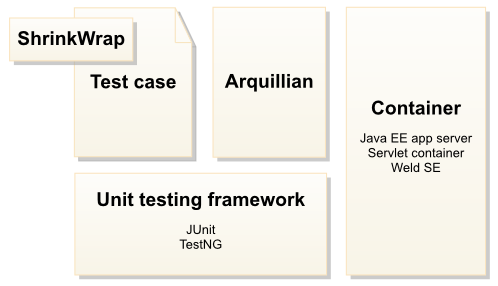
\includegraphics[width=80mm]{img/architecture-overview.png}
	\caption{The Arquillian test infrastructure}
	\label{fig:arquillian_test_infrastructure}
\end{figure}

	\section{Arquillian containers}
	
Arquillian container is an abstraction used in Arquillian context for a place where application we want to test (deployment) is deployed. Since Arquillian targets Java EE environment, a container is an enterprise application container such as JBoss AS\footnote{http://www.jboss.org/jbossas}, Glassfish\footnote{https://glassfish.java.net/} or similar.

Arquillian interacts with containers via so called \textit{container adapters}. Container adapter is a Maven dependency which implements specific Arquillian SPI and it is able to bridge communication from Arquillian to concrete container implementation. Maven container adapter implementation dependency has to be \texttt{test} scoped so it is present at class path during tests. Every container behaves differently when it comes to deploying, running and undeploying of an application. So then, every container has to have its own container adapter.

Arquillian recognizes three ways how to deal with containers: 
	
\begin{itemize}
	\item{Remote container - represents separate JVM where a container runs. Arquillian just connects to this kind of container in order to manage test execution. Life cycle of such container itself is not managed by Arquillian.}
	\item{Managed container - Arquillian controls the whole life cycle of a container, starting, stopping and deploying of an application under the test. This is basically the same case as remote container is. The only difference is in starting and stopping of a container. Arquillian manages it itself. A managed container is stopped after test execution is done. Same pays for its start.} 
	\item{Embedded container - resides in the same JVM as Arquillian does.}
\end{itemize}	

Every container adapter has to implement \texttt{DeployableContainer}\footnote{in org.jboss.arquillian.container.spi.client.container package} interface. Currently, there is allowed to be only one container implementation on the class path at the same time.

	\section{Arquillian descriptor}

When involving Arquillian into our project, there has to be a possibility to configure internals of Arquillian. The configuration is happening in a dedicated file called \texttt{arquillian.xml}\footnote{placed in src/test/resources when using Maven-like project}. This file serves as a central and the only one configuration file from where Arquillian reads all necessary information in order to be able to fire tests.

The selection of the container for our tests is happening at runtime, as mentioned before. Arquillian picks the right implementation according to container adapter which is present on the runtime class path when tests are executed. The very simple form of \texttt{arquillian.xml} could look like follows:

\lstinputlisting[language=XML,label=pop-pipe,caption=Simple arquillian.xml]{src/arquillian_simple.xml}

In this example, we specified two containers. Their appropriate dependency (container adapter) in \texttt{pom.xml} is added to the class path. Arquillian registers two containers (\texttt{jbossas-A} and \texttt{jbossas-B}). Both of them implement same container interface. We can define any number of containers (of the same kind). 

	\section{Anatomy of an Arquillian test}
	
After the explanation of the concept of a container and its selection during runtime, a form of an Arquillian test will be given. Arquillian test reuses JUnit testing principles heavily. After describing of Arquillian test in general, we will discuss the deployment modification, the negotiation of the test execution, the implementation of the communication between container and Arquillian and the test enrichment as well.

		\subsection{Arquillian test}

Arquillian test uses different test runner from JUnit test. Arquillian uses \texttt{Arquillian}\footnote{in org.jboss.arquillian.junit package} runner. Then all specifics of JUnit testing are the same but one. We have to create our custom deployment which is going to be deployed upon test execution to a container.

\lstinputlisting[language=Java,label=pop-pipe,caption=Arquillian test example]{src/arquillian_simple_test.java}	

Deployment is constructed in a method annotated with \texttt{@Deployment}. Deployment can also have a name as its annotation argument. This method has to be public and static. Deployment method returns an \texttt{Archive<?>}\footnote{org.jboss.shrinkwrap.api package} from previously described ShrinkWrap tool. Creation of a deployment this way is called \textit{micro deployment}. We do not ship the whole application. We are deploying only the very needed classes and resources so we are sure no other resources and functionality will be clashed. We assure the test case isolation.

Deployment, which is constructed programmatically, is meant to be deployed to container specified in \texttt{arquillian.xml}. Since we can use multiple containers, there can be more then one deployment method. In order to be able to recognize to which container some particular deployment is meant to be deployed, we have to use \texttt{@TargetsContainer} at deployment methods. The argument of this annotation is a qualifier we used previously in \texttt{arquillian.xml} when we were defining containers.

After deployment methods, tests, as we are used, are following. Since there can be more then one container configured, we are obliged to make difference between them, to specify on which container some particular method should run. Putting \texttt{@OperatesOnDeployment} annotation on \texttt{@Test} method, which argument is the name of a \texttt{@Deployment} method, ensures that this method will be executed in the right container.
		
		\subsection{Test deployment enrichment}

The very first thing the client side of Arquillian does is the modification of our deployment as we constructed it in our \texttt{@Deployment} method. This task is delegated to \texttt{DeploymentPackager}\footnote{in org.jboss.arquillian.container.test.spi.client.deployment package} SPI implementation. \texttt{DeploymentPackager} is responsible for the final deployment creation. Additional archives we are bundling into deployment are created in implementations of \texttt{AuxiliaryArchiveAppender}\footnote{in org.jboss.arquillian.container.test.spi.client.deployment package}. We can further process modification of archives we added via \texttt{AuxiliaryArchiveProcessor}\footnote{in org.jboss.arquillian.container.test.spi.client.deployment package} which is called once for every found \texttt{AuxiliaryArchiveAppender}.

Arquillian uses this SPI for adding of JUnit archive which is needed in order to be able to execute tests in the container context. It also adds other resources as, for example, \texttt{beans.xml} file into Java EE modules.

		\subsection{Test execution negotiation}

After Arquillian creates deployment via test's \texttt{@Deployment} method, it must deploy the archive and negotiate the test execution within a container. This task is let on SPI interface \texttt{ContainerMethodExecutor}\footnote{in org.jboss.arquillian.container.test.spi package} by which implementation we invoke test methods of our test class. These test method execution requests are delegated from the client side to \texttt{ServletTestRunner}\footnote{in org.jboss.arquillian.protocol.servlet package}. This class is bundled into deployment, as stated in the previous section. The method name and its class are specified as parameters to \texttt{ServletTestRunner}.

After servlet runner receives a message regarding test method invocation, it delegates to \texttt{TestRunner}\footnote {in org.jboss.arquillian.container.test.spi package} SPI implementation. The role of \texttt{TestRunner} is to dynamically build a test suite from a test class and run the suite subsequently. This work flow is happening in the container context.

The execution of test methods via \texttt{TestRunner} is happening subsequently. \texttt{TestRunner} has to let know the client side about the successful or unsuccessful result of test method execution. This information is translated, in container context, into \texttt{TestResult}\footnote{in org.jboss.arquillian.test.spi package} SPI implementation. The result is encoded (serialized) and sent back to the client side to \texttt{ContainerMethodExecutor}.

As we see, the test execution is performed dynamically over the network. Arquillian client side communicates with the test which is being invoked in container context. After test method execution, the result is sent back to client side. From the user point of view, he sees that test execution is being performed as he normally expects, knowing nothing about actual test execution over the network. 

		\subsection{Test class enrichment}	

Test enrichment is the process when resources are injected into a test class. The enrichment satisfies injection points by which we can in turn access and use injected members in test methods, avoiding their mocking. By injecting resources into test class within the container context, we are dealing with exactly the same resources as upon production-like usage.
 
Test enrichment of the test class is happening before the actual execution of test methods. We can enrich test class by annotating members of test class by annotations. Arquillian is supporting four ways how to inject a resource into the test class.

\begin{itemize}
\item{@Resource - use to inject Java EE resource injections}
\item{@EJB - used to inject EJB session beans}
\item{@Inject - used to inject CDI injections}
\item{@ArquillianResource - used to inject nonstandard, custom resources specified by Arquillian}
\end{itemize}

\texttt{@ArquillianResource} injection is supported via implementation of \texttt{ResourceProvider}\footnote{in org.jboss.arquillian.test.spi.enricher.resource package} SPI. We can then inject our own resources in the test case as simply as

\lstinputlisting[language=Java,label=pop-pipe,caption=Custom test enrichment]{src/enrichment.java}

	\section{Arquillian running modes}
	
Arquillian tests run in two modes. They are called \textit{client mode} and \textit{in-container} mode. They are defining the difference how tests are handled from the container point of view. The explanation of their differences is following.

		\subsection{In-container mode}
		
When testing by in-container mode, we are deploying our \texttt{@Deployment} directly into some container and tests are executed in that container - results of the tests are communicated back to Arquillian. By this way, we are testing how our deployment is doing while operating in container context. Arquillian uses in-container mode by default. However, the fact we want to run tests in container is set by \texttt{@Deployment(testable = true)} on our deployment method.

When we want to test in a container, we have to repackage our \texttt{@Deployment} every time so we are able to communicate with tests which are running in other JVM (when taking remote or managed container adapters into consideration). Communication is carried out via Servlet 3.0 protocol by default for Java EE 6 compliant application servers. 

		\subsection{Client mode}

Client mode does not repackage our \texttt{@Deployment} at all. A deployment is just sent to container "as-is" meaning no other modifications are done upon it. We are running tests outside of container. This mode is useful when we want to see how client would eventually use the application which is deployed in a container from his point of view. This running mode is not used by default - we set it by \texttt{@Deployment(testable = false)}.

		\subsection{Mixing running modes}

It is possible to mix running modes in one test class. When we use \texttt{@Deployment(testable = true)}, deployment is specified and tests are meant to be run in a container. However, when we do want to test from outside of a container, we have to use \texttt{@RunAsClient} annotation on a specific \texttt{@Test} method. By this way, we can assert some service is created in one test (doing it in container context) and we can as well assert that it behaves correctly from client point of view when we interact with this service in \texttt{@Test @RunAsClient} methods.

	\section{Arquillian event model}
	
Under the hood, Arquillian is event driven. There is a concept of \textit{events} which are \textit{fired}. All registered \textit{observers} which listens to such kind of events execute appropriate methods which listen to some specific kind of event. Event model is tree-like structure. The control is not returned to the initial point of fire until all subsequent logic is executed as well. Events can be chained, meaning when one event is fired and some method listens to it (via \texttt{@Observes} as argument annotation of event to handle), that method can fire another event to which other method of some observer is listening as well.

From the implementation point of view, events to be fired are classes. Events directed to be fired are created by injection into class from where firing is occurring. The firing itself is performed on the instance of created event via its \texttt{fire} method. The argument of firing method is new instance of class to be fired.

\lstinputlisting[language=Java,label=pop-pipe,caption=Injecting of event and firing it]{src/events.java}
	
	\section{Injection of classes}

In connection with event model which is embedded in Arquillian by default, question about flow of resources we create arises. When we pass the control from one method to another by events, there has to be a way how already existing instances of classes are accessed in them on demand.

Instances of classes we want to register into Arquillian for further usage are created via \texttt{InstanceProducer}\footnote{in org.jboss.arquillian.core.api package}. Let's say we need to register instance of \texttt{SomeClass} for further usage. The following example shows how this is achieved:

\lstinputlisting[language=Java,label=pop-pipe,caption=Instance producer in practice]{src/instance_producer.java}	
	
Instance producer just sets instance of class to be reached Arquillian-wide via its \texttt{set} method.

After class is instantiated and registered via its instance producer, we can access this instance wherever we want (logically only after time it is created) by \texttt{Instance}\footnote{in org.jboss.arquillian.core.api package} variable in class of access. Let's say we need to access instance of class we just produced and registered in the previous example. The following use case shows how to access this instance:

\lstinputlisting[language=Java,label=pop-pipe,caption=Access to produced instance]{src/instance_access.java}	

We get instance of \texttt{SomeClass} by \texttt{get} method. We can register only one instance of some particular class. Currently, there is no possibility to register multiple of them simultaneously because they are registered in \texttt{HashObjectStore}\footnote{in org.jboss.arquillian.core.spi package} which uses just \texttt{ConcurentHashMap<Class<?>, Object>} to store them.

Instances of classes we registered have their \textit{scope}. A scope of classes says during which period they are visible to be used and accessed. Scope of classes are defined during \texttt{InstanceProducer} declaration by using appropriate annotation. There are multiple scopes we can use for our instance producers. For the sake of argument, when we want to isolate the availability of some instance only during the period of container existence, we can do so by annotating instance producer with \texttt{ContainerScoped}\footnote{in org.jboss.arquillian.container.spi.context.annotation package}. The example follows:

\lstinputlisting[language=Java,label=pop-pipe,caption=Container scope example]{src/instance_container_scoped.java}

Instance producers and usage of appropriate scope is the feature Arquillian relies heavily on. Because of event nature and behavior of Arquillian framework, producing of instances is essential part without which we could control instance passing very inconveniently.

	\section{Extensibility of Arquillian}

Arquillian uses concept of SPI heavily so in order to override some functionality or to add our own, we have to register our custom implementation of SPI interfaces into Arquillian. These implementations then override defaults, incorporating our own functionality directly into core Arquillian infrastructure.

Arquillian is extend by \textit{extensions}. An extensions is distributed as a Maven dependency. In order to recognize an extension from Arquillian point of view, an extension has to specify the access point to it. The name of a class which implements \texttt{LoadableExtension}\footnote{in org.jboss.arquillian.core.spi package} SPI has to be placed in the file of the same name in \texttt{src/main/resources/META-INF} folder in the extension module.

Concrete implementations of SPI interfaces are registered in the implementation of \texttt{LoadableExtension} in \texttt{register} method. Classes are registered via \texttt{LoadableExtension.ExtensionBuilder}. To pick the most important methods, these are \texttt{observer}, for registering classes which observe for events, and \texttt{service}, for registering classes which are able to produce instances to be injected into other classes.

	\section{Conclusion}
	
In the previous sections, overall functionality and principles of Arquillian testing platform were given. The reader should have solid background regarding principles of Arquillian and he should also grasp main features and architectural design when it comes to test negotiation, test enrichment, container abstraction and Arquillian extensibility.

The incorporation of Arquillian framework into testing process of Java EE application is more than welcome. Arquillian provides other way how we can look at testing. Testing is becoming the essential part of development so it is very suitable for programming styles as XP or iterative development processes in general. By possibility of trying our code directly in target environment, testing process becomes central activity to focus on.

\chapter{Arquillian Android container}

After the presentation of the two mainstream development processes and the justification of the necessity of continuous integration, the reader could make himself familiar about various tools needed and used in Java EE environment which usage shows vector how a developer can code Java EE applications effectively.

The last chapter dealt with describing of main features of Arquillian testing platform. The reader is aware of advantages of Arqullian testing platform in Java EE environment and sees advantages of using Arquillian in testing process of (not only) Java EE applications by XP or iterative way.

In this chapter, we are going to describe reasons and the development model of Java EE application based on Android platform. We then conclude that there is a need for Arquillian Android container which will be subsequently designed and implemented in upcoming chapters.

	\section{Central ideas}

As we saw, the central concept around which Arquillian is turning around is the concept of \textit{container}. Container abstraction serves as a common pattern how application is deployed and how tests are executed afterwards.

As described previously, the support for a container is implemented via container adapter. A container adapter is a Maven dependency which, once on class path, it is able to communicate with Arquillian on one side and with concrete container implementation on the other side.

When we want to bring the whole testing idea from ordinary Java EE environment into Android platform, taking into consideration container abstraction, we clearly see that Android device itself could be viewed as container to which applications are deployed and the whole principle of testing could be just the same. Since deployment is a term used for Java EE containers, we will use term \textit{installation} instead.

Testing of applications is divided into two categories. We can test web applications and native Android applications.

Regarding web applications, it is clear that they are not going to be run on Android device itself. Web applications are deployed in ordinary application containers as we are used. However, when executing tests, web application or its part from \texttt{@Deployment} has to be deployed in web application container but tests have to be executed from Android point of view, in browser which runs on Android device, against the web deployment.

This approach brings the basic problem in supporting of multiple adapter containers on the class path. As explained previously, we can specify only container (even multiple of them) of the same kind. Next, we have to figure out how testing will be carried out. We need to bring Selenium into Android context.

Regarding native Android application, we need to do the investigation how Android container could support writing tests in a similar way as Selenium is doing with web browsers. Selenium and its extensions as WebDriver operates with web elements. When testing native Android applications, we need to operate on elements by which application is built as such.

Last but not least, we need to implement the whole Android container. Android container is working with two types of containers. One type of container stands for virtual device called \textit{Android Virtual Device (AVD)} from Android SDK. The other one is real physical Android device (e.g. a mobile phone).

It is necessary to support both types of devices from developer point of view so he uses Android device transparently - it does not matter if there is emulated or real device underneath. 

Since we strives for having only one implementation of Arquillian Android container and we need to support web testing as well as native testing of Android applications, we have to provide a way how to achieve this desire. 

Arquillian Android container has to be \textit{testing agnostic}, meaning the decision about the way of testing (web or native mode) is the decision resolved upon runtime. Whichever implementation of testing mode will be present on class path during testing process, that testing mode will be used.

Supporting both modes of testing while having one kind of container leads to the necessity of implementing Arquillian Android container in a pluggable way. By this solution, we are opening doors for other kind of testing implementation which developer could deliver for Arquillian Android container, preserving its extensibility.

	\section{Architectural decisions}

Arquillian Android container\footnote{expression "Android container" will be used from now on for brevity} is managed container. Managed containers, as described earlier, are containers which life cycle is controlled and initiated (like start and stop of container) by Arquillian itself.

Android container is in some sense remote container as well. We need to be able to connect to running AVD instances as well as to some real physical device which is already up and running independently from us. In this case, we should use term \textit{remote container} instead of managed but we prefer managed version more since connecting to already running container is just a feature of the container logic as such.

Android container is a Maven-based Java application which implements container abstraction of Arquillian testing platform. From the Maven point of view, Android container is divided into modules which combined together shapes the whole container implementation.

At high level, Android container consists of these Maven based sub-projects (by alphabetical order):

\begin{itemize}
	\item{\texttt{android-container-api}: contains API for Android container, interfaces to be implemented for \texttt{arquillian-android-managed} implementation}
	\item{\texttt{android-container-bom}: Bill of materials for Android container}
	\item{\texttt{android-container-build-config}: contains configuration files to import into IDE (Eclipse\footnote{http://www.eclipse.org/}-based) for following JDF\footnote{http://www.jboss.org/jdf/} coding style. Arquillian fits under JDF and JBoss universe as Arquillian Android container does. JDF offers various configuration files to import to IDE for coding style and source code formatting. Arquillian Android container follows these guidelines so it is JDF and JBoss compliant.}
	\item{\texttt{android-container-build}: specifies dependency management and configuration of plugin executions such as Maven compiler plugin for project's build.}
	\item{\texttt{android-container-depchain}: aggregates all implementation modules in case they are needed in other project}
	\item{\texttt{android-container-managed}: introduces the central implementation of the Android container.}
	\item{\texttt{android-container-spi}: implements classes for events to be fired to control execution path for Android container}
	\item{\texttt{android-multiple-containers}: implements custom implementation of container registration for Arquillian so more than one container adapter can be present at class path during runtime}
	\item{\texttt{pom.xml}: aggregates all modules, serves as a parent via which the whole project is built, packaged and installed.}
\end{itemize}

To reflect parent-child relationship from the Maven point of view, the following figure~\ref{fig:android_container_maven_modules} captures Android container modules and this relationship.

From the design point of view, Android container execution flow is event-driven which means the flow from one part of program to another is based on message passing as described previously. By designing Android container this way, Android container is highly modular. There is not spaghetti-like code not only because of objected oriented approach but also because we can isolate the responsibility of implementation classes very easily and precisely.

By event-driven approach, extensions of Android container are written relatively easily as well. Even if we do not know how particular functionality will be implemented by future extensions, by firing and observing events we are providing extension points the third party software can rely on. Android container just offers these events to be observed, processed and fired back. Since firing of messages directs execution flow, integration of external extensions which have to be put on class path at runtime guarantees that Android container is pluggable.

\begin{figure}[h!tb]
	\centering
	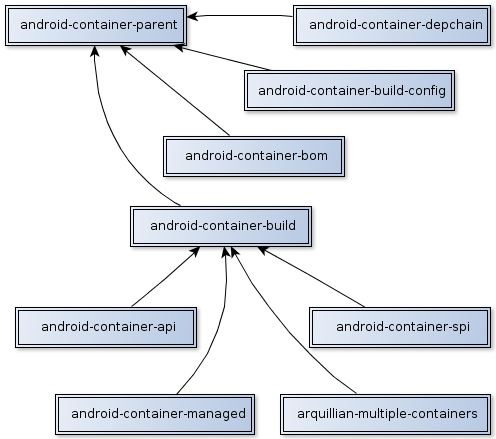
\includegraphics[width=.8\textwidth]{resources/android-container-modules.png}
	\caption{Arquillian Android container - Maven modules}
	\label{fig:android_container_maven_modules}
\end{figure}

\chapter{Implementation of Arquillian Android container}

It is clear that we have to interact with actual Android device in some way. Android container is just a layer between Arquillian and Android device. The interface of Android device we can communicate with is implemented in Maven library called \texttt{ddmlib}\footnote{com.android.ddmlib:ddmlib}. \texttt{ddmlib} is Java library for communication with Android device and Android Debug Bridge to which Android device is connected. We do not communicate with Android device directly but we do so via mentioned Android Debug Bridge. Every device is connected to so called \textit{console port}. We can execute various command via debug bridge, these are internally translated into corresponding commands and actions performed at Android device, virtual or physical.

In order to be able to arrange interaction with Android devices, there has to be Android SDK installed on the host computer. Android SDK bundles all existing versions of AVD\footnote{Android Virtual Device}, provides all commands for creating AVD, starting emulator, creating Android SD card and so on. It is crucial to have Android SDK installed on host computer when testing. Without Android SDK, it is not possible to bring Android into our tests. The existence and presence of Android SDK is tested in Android container. Its location is typically reflected by \texttt{ANDROID\_HOME} system property, it can be changed in container configuration to any arbitrary location.

	\section{Extension for multiple containers}

In order to suppress the limitation of Arquillian container abstraction - using only one implementation of \texttt{DeployableContainer} on the classpath at time - there is the module \texttt{arquillian-multiple-containers} implemented. The very first thing which Arquillian does while executing the testing lifecycle is to read Arquillian descriptor in \texttt{arquillian.xml} and figure out which containers are about to be registered.

In \texttt{arquillian-multiple-containers} module we are suppressing the implementation of \texttt{ContainerExtension}\footnote{in org.jboss.arquillian.container.impl package} and we are providing \texttt{MultipleContainersExtension}\footnote{in org.jboss.arquillian.extension.multiplecontainers package} implementation instead. The fact \linebreak about taking other container extension implementation into consideration is fulfilled via SPI mechanism in \texttt{META-INF/services/}\footnote{in org.jboss.arquillian.core.spi.LoadableExtension} configuration file. 

\texttt{MultipleContainerRegistryCreator} class observes event \linebreak \texttt{ArquillianDescriptor} from Arquillian. It scans for all available container definitions in \texttt{arquillian.xml}, then it creates container register of \texttt{MultipleLocalContainersRegistry} and registers newly scanned containers via its \texttt{create} method. Definitions of containers in Arquillian descriptor in \texttt{arquillian.xml} are validated, so e.g. there can not be more than one default container or group of containers.

During actual creation of concrete container, container registry (via its \texttt{create} method) loads all implementations of \texttt{DeployableContainer} located on class path and then compares configuration property named \texttt{adapterImplClass} in container definition against already loaded implementations. If match is found, such container is created via \linebreak \texttt{addContainer} method.

It is worth to say that \texttt{adapterImplClass} property has to be defined in container configuration in \texttt{arquillian.xml} only in case when more then one different \texttt{DeployableContainer} implementations are on class path. We can omit its presence when one implementation is on class path because there is not ambiguity anymore. 

	\section{Configuration}
	
After being able to register more than one container implementation of \texttt{DeployableContainer}, so JBoss AS container (or any other container) can live besides Android container transparently, we have to configure these containers. The focus on the configuration of Android container will be given since configuration of other containers is out of scope.

Configuration of Android container is defined by implementations of \texttt{ContainerConfiguration}\footnote{in org.jboss.arquillian.container.spi.client.container package}, in our case - \texttt{Android\-Managed\-Container\-Configuration}\footnote{in org.jboss.arquillian.container.android.managed.configuration package} class. Values of configuration properties are automatically scanned from \texttt{arquillian.xml} and dynamically put into their corresponding class members in configuration class.

Validation of all configuration properties is executed via \texttt{validate} method of configuration class. The complete documentation of the container configuration can be found in resources.

	\section{Implementation of container lifecycle}	
	
We start the explanation of Android container implementation with the most crucial class the whole container lifecycle is turning around - \texttt{AndroidManagedDeployableContainer}\footnote{in org.jboss.arquillian.container.android.managed package}. All container implementations have to implement \texttt{DeployableContainer} interface as this class does. The lifecycle of any container (so Android container as well) can be described in the following flow, names of these actions are exactly names of methods of \texttt{DeployableContainer} to be overridden:

\begin{itemize}[nolistsep]
	\item{\texttt{setup} - sets up a container, e.g. its configuration passed as the argument is treated appropriately and additional steps required to be done before actual starting of a container are figured out}
	\item{\texttt{start} - starts a container, this method starts container from scratch in case of managed container or it can provide a way how to connect to already running container in case of remote container}
	\item{\texttt{deploy} - deploys an archive assembled in \texttt{@Deployment} in the test class}
	\item{\texttt{undeploy} - undeploys an archive which was previously deployed to container}
	\item{\texttt{stop} - stops container, in case of managed container it means its shutdown, in case of remote container it basically means that we disconnect from it safely after deployment is undeployed and test results are returned back to us}
\end{itemize}

When setting up Android container in \texttt{setup} method, first of all, Android container configuration \footnote{AndroidManagedContainerConfiguration class} is made \texttt{@ContainerScoped} via its \texttt{InstanceProducer} injection point. By doing this, we can access Android configuration during the whole Android container lifecycle via normal \texttt{Instance} injection in any class which needs the access to Android container configuration from \texttt{arquillian.xml}.

This pattern of creating resources via instance producers is typical in Android container and will be visible many times now on. The usage of annotation as \texttt{@ContainerScoped} is needed because injection producers makes these classes visible during the whole lifetime of the application and that is not desired because when we start another Android container, that class would take over the new one. All instance producers creates instances which are \texttt{@ContainerScoped} for the same reason.

We set \texttt{AndroidSDK}\footnote{org.jboss.arquillian.container.android.managed.configuration package} instance which abstracts the interaction with Android SDK installation on our host in the same way. After preparing all needed to start the container itself, Arquillian proceeds and executes \texttt{start} method.

		\subsection{Starting of a container}

			\subsubsection{Emulator}
	
			\subsubsection{Physical device}
	
		\subsection{Deploying and undeploying}
	
		\subsection{Stopping of a container}

		\subsection{Android SD card}
	
	\section{Usage}

After the explanation of the internal workings of Android container, we are going to show	 possible use cases how Android container abstraction can be used. Various scenarios are discussed.

We start with the presentation of a simple Android container test which runs tests as a client. After that, we show how Android container can be used in connection with other type of container e.g. JBoss AS. This use case shows how different container adapter implementations can be put in one test because of arquillian-multiple-containers extension. In the end, the example of executing tests in two different Android containers will be given.

In any case, when we want to test with Android container, we have to put its container adapter on class path as mentioned early for any other container. In our case, we have to add the dependency \texttt{android-container-depchain}\footnote{org.jboss.arquillian.container:android-container-depchain:pom} with \texttt{test} scope as a Maven dependency into \texttt{pom.xml} of our test project.

		\subsection{Android container test}

Our test case review starts with a simple Android container test execution. The test is going to be run as the client test. Since every Arquillian test has to have \texttt{@Deployment} method, we create a dummy archive which would be installed (unmodified because of \texttt{@RunAsClient} annotation on class) on the injected \texttt{@AndroidDevice} instance.

These kinds of tests are useful when using just \texttt{AndroidDevice} and its methods alone. We do not have any additional plugins on class path but Android container itself so we can not modify deployment nor install it on the device. The deployment method has to be specified since it is there for the completeness and satisfaction of Arquillian API.

\lstinputlisting[language=Java,label=pop-pipe,caption=Android container test]{src/android_test_01.java}

		\subsection{Mixed container adapters test}

By mixing different container adapter implementations, we can achieve testing against two containers in one test. We have to add ordinary container adapter on class path and specify class which implements \texttt{DeployableContainer} interface in \texttt{adapterImpl} property in \linebreak \texttt{arquillian.xml}. When we want to use e.g. Android container and JBoss AS, we need to put both adapter dependencies in Maven's \texttt{pom.xml}. \texttt{arquillian\--multiple-containers} takes care of registering these two container implementations into Arquillian. After that, we can create two deployment methods which match described containers and we can run tests against these deployments afterwards as expected.

\lstinputlisting[language=Java,label=pop-pipe,caption=Mixed container adapters test example]{src/android_test_02.java}
	
It is important to say that we have to put \texttt{@ArquillianResource} as \texttt{test01} method argument since this class "runs" in both containers so this injection point could not be satisfied at JBoss AS side. Android device is \texttt{@ContainerScoped} so when another container takes over, instance of the Android device is no more visible. This injection point has to be recognized only in the Android context. We achieve this by adding \texttt{@OperateOnDeployment} annotation which targets our container on the test method.

		\subsection{Multiple Android containers test}

The last example how Android container can be used is dedicated for showing two Android containers in one test. When a user wants to use multiple \texttt{AndroidDevice}s, he has to specify against which deployments and containers these tests have to be executed. Once again, we are using client running mode.  

\lstinputlisting[language=Java,label=pop-pipe,caption=Multiple Android containers test]{src/android_test_03.java}

It is important to note that we are using just one injection point but every test method has its own instance of \texttt{AndroidDevice} injected (so container), for \texttt{test01} there is \texttt{android1} device injected but for \texttt{test02} there is \texttt{android2} device used.

\chapter{Integration of web testing}

	\section{Arquillian Android Drone for web testing}

\chapter{Investigation for native testing}

	\section{Arquillian Android Drone for native testing}

\bibliographystyle{plain}  % bibliografický styl 
\bibliography{bib-db}      % soubor s citovanými
                           % položkami bibliografie 

\printindex

%%%%%%%%%%%%%%%%%%%%%%%%%%%%%%%
%
%       A P P E N D I X  
%
%%%%%%%%%%%%%%%%%%%%%%%%%%%%%%%

\appendix
\end{document}
